\documentclass{article}
%\setlength{\mathindent}{0pt}
% Package for better handling of figures
\usepackage{graphicx}
% Package for better handling of tables
\usepackage{array}
% Package for better handling of mathematical symbols
\usepackage{mathrsfs}
\usepackage{amsmath}
\usepackage{amssymb}
\usepackage{multirow}
\usepackage{array}
\usepackage{float}


% Title and Author Information
\title{Privacy-Preserved Meeting Organization}
\author{Group 06}
\date{\today} % You can specify a different date if needed

\begin{document}

% Title Page
\maketitle

% Tentative basic definitions
\section{Basic definitions}

\noindent
Following finite sets are defined:
\begin{itemize}
    \item $\mathcal{D}$: The set of all documents.
    \item $\mathcal{R}$: The set of all roles.
    \item $\mathcal{I}$: The set of all individuals
    \item $\mathcal{L}$: The set of all locations.
    \item $\mathcal{T}$: The set of all time slots.
\end{itemize}

% Access Control List
\section{Access Control List}
\noindent
We define following relationships, using above definitions.
\[ d = \{ d \in \mathcal{D} \mid \text{d is a document} \} \]
\[ i = \{ i \in \mathcal{I} \mid i \text{ is an individual } \} \]
\[ g = \{ g \subseteq \mathcal{I} \mid g \text{ is a subset of one or more individuals in } \mathcal{I} \} \] \\ 
\noindent
Above relationships mean that $d$ is an element of set $\mathcal{D}$, and $i$ is an element of set $\mathcal{I}$. Further, $g$ is a group of one or more individuals ($i$), where $i \in \mathcal{I}$, such that $g \ne \emptyset$.\\ 

\noindent
Consider that following finite set is also defined:
\begin{itemize}
    \item $\mathcal{G}$: Set of all possible not-null subsets of $\mathcal{I}$
\end{itemize}
Based on above all sets, we define following relationship.
\[ access(d) = \{ g \in \mathcal{G} \mid g \text{ has access to } d \} \] \\ 
\noindent
Above relationship means that $g$ is an element of set $\mathcal{G}$, and that $access(d)$ is the set of groups ($g$) having access permission to document $d$.\\ 
Here we note that, $access(d) = \mathcal{G}$ converts $d$ to a \textbf{public document}. \\ 

By above last two relationships, since any element $g$ of $access(d)$ is also a subset of $\mathcal{I}$, such that $g \subseteq \mathcal{I}$, we have the relationship $access(d) \subseteq \mathcal{I}$, when $access(d)$ is defined in form of \textbf{singleton subsets} of $\mathcal{I}$. It implies also that $|access(d)| \leq |\mathcal{I}|$, when $access(d)$ is defined in the form of singleton subsets of $\mathcal{I}$. Simply, a singleton subset of $\mathcal{I}$ includes an individual ($i$).  \\
Regarding that inequality, $|access(d)| = |\mathcal{I}|$ is the situation when every $i$ in $\mathcal{I}$ is present in at least one group ($g$), such that $g \subseteq access(d)$. At such a situation, both relationships $access(d) = \mathcal{G}$ and $|access(d)| = |\mathcal{I}|$ imply the same meaning that, document is a \textbf{public} document.\\ \\

% Meeting agenda
\section{Meeting agenda}
\noindent
Agenda of a meeting is the document that defines the set of groups ($g$) required to attend the meeting, where \textbf{group} has same meaning as defined above.
When we consider agenda as document $d$, those groups ($g$) are elements of set $access(agenda)$.\\ \\
Theoretically it is possible to require all individuals of set $\mathcal{I}$ or all available not-null subsets of set $\mathcal{I}$, to attend a single meeting. But, in practical scenario, probability of organizing such a meeting is low. \\ \\

However, there are both private meetings and public meetings, in our scope. If $access(d) = \mathcal{G}$ is used for meeting agenda of public meetings, it's impossible to distinguish the intended participant groups explicitly. Therefore, in agenda document of public meetings, we include a group labeled as \textbf{public} group, in addition to the actual intended participant groups of meeting, to state that agenda is \textbf{public}. So, on the other hand, absence of group labeled as \textbf{public} in $access(agenda)$ means that, meeting is \textbf{private}.
\begin{itemize}
    \item If there is at least one document in meeting, such that $access(d) \ne \mathcal{G}$, \textbf{public} group shouldn't have access to meeting agenda.
    \item If every documents in meeting has $access(d)$ such that $access(d) = \mathcal{G}$, \textbf{public} group can have access to meeting agenda.
    \item If agenda is the only document in meeting, \textbf{public} label can be used by meeting organizer to define whether agenda document is \textbf{private} or \textbf{public} (i.e. whether meeting is private or public).
\end{itemize}

\noindent
Following flow chart depicts the process of identifying whether a document is \textbf{private} or \textbf{public}.
\begin{figure}[H]
    \centering
    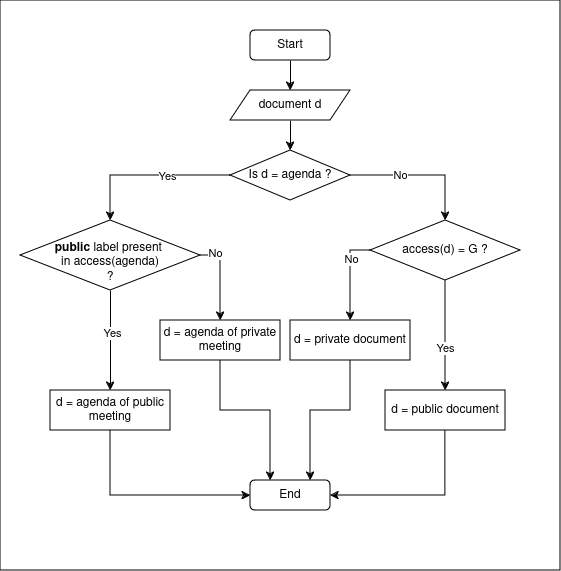
\includegraphics[width=0.7\textwidth]{./image/document_puclic_vs_private_classification.png}
    \caption{Process to identify whether a document is private or public}
    \label{fig:sample}
\end{figure} 

\noindent
Regarding other documents except agenda, for simplicity of implementation, we can include only \textbf{public} label in access control list, without including any other group of $\mathcal{G}$, to mean that $access(d) = \mathcal{G}$ or that document is a public document. Because, we do not need to include any other group ($g$) in a public non-agenda document, though we required them in public agenda documents for identifying meeting participants.\\ \\
\noindent
In addition to presence or absence of \textbf{public} label in $access(agenda)$, meeting agenda should define the \textbf{meeting quorum}, for the meeting. This theme will be discussed later.

% Definition of a meeting
\section{Definition of a meeting}

\noindent
\textbf{We assume that every meeting has an agenda associated with it, to define the set of groups($g$) required to attend the meeting}. Agenda of a particular meeting $M$ is a document, belonging to set $\mathcal{D}$.\\ \\
When we consider the agenda document of meeting $M$, for every group $g$ invited to meeting $M$; $g \in access(agenda)$. Also consider that, $D$ represents set of documents discussed in $M$, including agenda, such that $D \subseteq \mathcal{D}$. Hence, according to the assumption emphasized above, for any meeting $M$; $|D| \geq 1$.\\ \\ 
For conducting a meeting, at least 2 individuals are required. Consider that $I$ represents the set of individuals attending meeting $M$, such that $I \subseteq \mathcal{I}$, when groups ($g$) of $access(agenda)$ are converted to corresponding elementary individuals ($i$). Here we note that, for any meeting $M$; $|I| \geq 2$.\\
Accordingly, when $access(agenda)$ is defined in terms of singleton subsets of $\mathcal{G}$, and those groups (singleton subsets) in $access(agenda)$ are represented by $G$, such that $G \subseteq \mathcal{G}$, it can be observed that $|G| \geq 2$. \\ \\  
Consider set of locations of individuals in $M$ as $L$ (in other words, set of locations of indiduals in set $I$, during meeting time), such that $L \subseteq \mathcal{L}$. Every individual attends meeting from a particular location $l$, such that $l \in L$. We note that, if meeting is online or hybrid, $|L| > 1$. If meeting is onsite, $|L| = 1$, since every individual is at same location. Every meeting should be in one mode, out of online, hybrid, onsite modes. Therefore, for any meeting $M$; $|L| \geq 1$. \\ \\
Since a \textbf{meeting} is a \textbf{synchrnous} communication, every individual in meeting $M$ should attend the meeting during the same time slot $t$ (Assuming that all individuals are in same time zone).  \\ \\
Based on these definitions, we define meeting M as a 4-tupple,
    \[ M = < D, I, L, t > \]
such that,
    \[ D \subseteq \mathcal{D} \]
    \[ L \subseteq \mathcal{L} \]
    \[ I \subseteq \mathcal{I} \]
    \[ t \in \mathcal{T} \]


% Transformation of individual into role
\section{Transformation of individual into role}
\noindent
Consider that same sets defined above will be used in explanations below, in same notations: \\ \\
\noindent
Consider $g$ and $g'$ as subsets of $\mathcal{G}$ such that $g, g' \subseteq \mathcal{G}$. And consider $d$ as a \textbf{private} document , $l$ as a location and $t$ as a time slot such that $d \in \mathcal{D}$, $l \in \mathcal{L}$ and $t \in \mathcal{T}$.
Further consider that $g \in access(d)$ and $g' \notin access(d)$, for restricting access of document $d$, where $|access(d)| = n$ , given that $access(d)$ is defined as a set of singleton subsets of $\mathcal{G}$. A singleton subset of $\mathcal{G}$ means an elementary subset $g$, in which only one element (i.e. only one individual $i$) is present.\\ 
Also note that, $i$ and $i'$ are two individuals representing subsets $g$ and $g'$, respectively. \\ \\
\noindent
Assume that at scenario 1, $i$ attends a \textbf{meeting} at location $l$ during time slot $t$ to discuss document $d$, where $i'$ has no access to location $l$ during same time slot $t$. \\
Here we state that privacy of meeting discussing document $d$ was preserved at context $l \times t$ \\ \\ 
\noindent
Now assume that at scenario 2, $i$ attends a \textbf{meeting} at location $l$ during time slot $t$ to discuss document $d$, where $i'$ also has access to location $l$ during same time slot $t$. \\
Here we state that privacy of meeting discussing document $d$ was violated at context $l \times t$, because $n + 1$ individuals including $i'$ have got access to content of document $d$. But actually $|access(d)| = n$, when $access(d)$ is defined as a set of singleton subsets of $\mathcal{G}$, as mentioned above. We observe that $(n + 1) \geq |access(d)| = n$ \\ \\ 
\noindent
When above 2 scenarios are compared, we observe that role of same individual $i$, representing subset $g$ such that $g \in access(d)$, has experienced a variation. Context of $i$ has changed, depending on location and time. \\ \\
Therefore we define that presence of $i$ at context $l \times t$ transforms $i$ to role $r$.
\[ transform(i, l, t) = r : r \text{ is role of } i \text{ at location } l \text{ at time slot } t \] 
\noindent
If $g \in access(d)$, $g' \notin access(d)$ and $d$ is a \textbf{private} document, $i$ representing $g$ should attend a meeting to discuss $d$ at context $l \times t$, only if $i'$ representing $g'$ has no access to $l \times t$. Accordingly, to identify the privacy preserving context for discussing document $d$, combination of i, l, t is required.\\ \\



% Difference between public and private roles
\section{Difference between public and private roles}
When we consider a \textbf{private} document $d$, we can't exactly predict the time, at which $i'$, representing $g'$, such that $g' \notin access(d)$, will get access to location $l$. 
Therefore, meeting organizer has the responsibility of defining location $l$ as a \textbf{private} location or a \textbf{public} location, considering whether access of $i'$ has been strictly restricted, during all potential meeting time slots (represented by set $\mathcal{T}$).\\ \\
Using this definition and above formula, we can show that, $i$ representing $g$, such that $g \in access(d)$ where $d$ is a \textbf{private} document, is transformed to role $g$ itself, at a \textbf{private} location. 
Here, location should be defined as a \textbf{private} location, by same entity, that defined the set $access(d)$ for document $d$.

\[ transform(i, l, t) = r \]
\[ transform(i, (private\_location), t) = r \]
\[ transform(i, (private\_location), t) = g \] \\

\noindent
On the other hand, any location $l$ is defined as a \textbf{public} location, if access of $i'$ has \textbf{not} been strictly restricted, during any potential meeting time slot in set of time slots $\mathcal{T}$.\\ \\
Using this definition and above formula, we can show that, $i$ representing $g$, such that $g \in access(d)$, is transformed to \textbf{public} role, at a \textbf{public} location.
Location should be defined as a \textbf{public} location, by same entity, that defined the set $access(d)$ for document $d$.

\[ transform(i, l, t) = r \]
\[ transform(i, (public\_location), t) = r \]
\[ transform(i, (public\_location), t) = public \] \\
\noindent
Based on these derivations, we have identified a constraint relevant to $i$, for discussing $d$ in a privacy preserved meeting.\\ \\
\textbf{Constraint}: When $d$ is a \textbf{private} document, every $i$ representing $g$, such that $g \in access(d)$, that attends a meeting to discuss document $d$, must represent role $g$ in the meeting.\\ \\
When $d$ is a \textbf{public} document, every $i$ that attends a meeting to discuss document $d$, is allowed to represent \textbf{public} role in the meeting.\\ \\

% Sub-section: Roles in meeting agenda
\subsection{Roles in meeting agenda}
\noindent
If meeting agenda document does not include the group labeled as \textbf{public} in $access(agenda)$, it means that $\textbf{public} \notin access(agenda)$. Then $i'$ representing $g'$ such that $g' \notin access(d)$, should be strictly prevented from accessing the meeting, by conducting meeting at a \textbf{private} location, defined by relevant meeting organizing entity.\\ \\
On the other hand, if meeting agenda includes group labeled as \textbf{public} in $access(agenda)$, it means that $\textbf{public} \in access(agenda)$. Then it is \textbf{not} mandatory to prevent access of $i'$ representing $g'$ such that $g' \notin access(d)$, for the meeting. Therefore, meeting can be conducted at a \textbf{private} location or \textbf{public} location, based on locations defined by relevant meeting organizing entity.\\ \\

% Variation of role
\section{Variation of role}
\noindent
Now consider a situation where individual $i$ representing $g$, such that $g \in access(d)$ has $x$ number of locations, out of which any one can be selected for attending a meeting to discuss $d$. And assume that $i$ has $y$ number of time slots, out of which any one can be selected for attending the meeting.\\ \\
We can depict the possible variations of $transform(i, l, t)$ function as below, for individual $i$, depending on locations defined by the entity, assuming that $i$ doesn't change location during middle of a time slot.
\begin{table}[H]
    \centering
    \begin{tabular}{|c|c|c|c|c|c|}
    \hline
    $(i)$ & $t_1$ & $t_2$ & $...$ & $t_{y-1}$ & $t_{y}$ \\
    \hline
    $l_1$ & x & x & \  & x & x \\
    \hline
    $l_2$ & x & x & \  & x & x \\
    \hline
    $...$ & \  & \  & \  & \  & \  \\
    \hline
    $l_{x-1}$ & x & x & \  & x & x \\
    \hline
    $l_{x}$ & x & x & \  & x & x \\
    \hline
    \end{tabular}
    \caption{Possibilities in variation of $transform(i,l,t)$ for individual $i$}
    \label{tab:six_columns_six_rows}
\end{table}

\noindent
Note that $l_x$ represents the $x^{th}$ location, while $t_y$ represents the $y^{th}$ time slot. Meanwhile x represents the role of $i$ at the corresponding $l$ and $t$ (based on formula $transform(i, l, t) = r$). According to this representation, we observe that $i$ has $x \times y$ number of possibilities at maximum, to attain the role.\\ \\
Here we emphasize that some x roles can be categorized as \textbf{public}, with respect to \textbf{public} locations defined by an entity. According to the constraint identified, if $d$ is a \textbf{private} document, $i$ should attend the meeting only when $r = g$, such that $g \in access(d)$. When r = \textbf{public} role, individual $i$ should strictly avoid discussing \textbf{private} documents. By following this constraint, access of $i'$ representing $g'$, such that $g' \notin aceess(d)$, into this meeting can be prevented.\\ \\ 

% Privacy-preserved meeting
\section{Privacy-preserved meeting}
Based on above descriptions and definitions, we define privacy-preserved meeting as below;\\
\textbf{A privacy-preserved meeting is a meeting in which, individual i representing role r has no access to the meeting, when $r = g$ and $g \notin access(agenda)$}.


% Meeting participant validation
\section{Privacy of documents}
\subsection{Participants in access control lists of non-agenda documents}
\noindent
It is possible to discuss one or more documents in a meeting. Further, there can be both public documents and private documents among these documents. We do not need to follow any constraint to protect the privacy of public documents.\\ \\
But when private documents are considered, it is needed to follow some constraints to pretect the privacy. For example, consider $d_{1}$ and $d_{2}$ as 2 private documents. An individual $i$ representing $r$, such that $r = g$ and $g \in access(d_{1})$, can be absent in access control list of $d_{2}$. In other words, $g \notin access(d_{2})$ relationship can exist.\\ \\
In this situation, discussing both $d_{1}$ and $d_{2}$ in same meeting can violate the privacy of $d_{2}$, when above mentioned indivisual $i$ participates in that meeting. It means that, for discussing both $d_{1}$ and $d_{2}$ in same meeting, roles of all meeting participants should mandatorily be present in both $access(d_{1})$ and $access(d_{2})$. This relationship is graphically depicted in diagram below.
\begin{figure}[H]
    \centering
    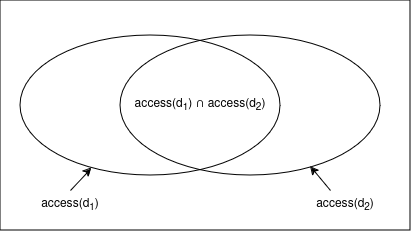
\includegraphics[width=0.7\textwidth]{./image/d1_intersection_d2.png}
    \caption{Intersection of access control lists of 2 private documents}
    \label{fig:sample}
\end{figure} 
\noindent
This concept is applicable not only for 2 private documents, but also for any number of private documents discussed in same meeting. When there are $n$ number of private documents to discuss in a meeting, intersection of access control lists of all those documents should be considered. Any individual $i$ such that $i \notin (access(d_{1}) \cap access(d_{2}) \cap ... \cap access(d_{n-1}) \cap access(d_{n}))$ should be prevented from accessing the meeting.
\subsection{Meeting participant validation}
\noindent
When there are private documents to discuss in a meeting, it is required to validate intersection of participants identified as above, with participants included in access control list of meeting agenda (see "Meeting agenda" section for more details on meeting agenda).\\ 
For protecting privacy of $n$ number of private documents defined as $d_{1}, ... , d_{n}$, following relationship must be satisfied for the meeting. 
\[ access(agenda) \subseteq \{access(d_{1}) \cap access(d_{2}) \cap ... \cap access(d_{n-1}) \cap access(d_{n})\} \]
\noindent
Simply, above relationship means that each and every individual $i$ representing role $r$, such that $r = g$ and $g \in access(agenda)$, is also an element of the intersection of $access(d)$ of all private documents discussed in meeting.
A situation in which above relationship is violated can be explained by using following relationship. 
\[ \{access(d_{1}) \cap access(d_{2}) \cap ... \cap access(d_{n-1}) \cap access(d_{n})\} \subset access(agenda) \]
In simple terms, above relationship means that there exists at least one $i$ representing $r$, such that $r = g$ and $g \in access(agenda)$, where $g$ is not an element in the intersection of $access(d)$ of all private documents discussed in meeting.\\ \\
\noindent
However, for discussing public documents in meeting, it is not required to perform any participant validation. In other words, any individual $i$ can discuss public documents, in any private or public meeting.


% Meeting quorum
\section{Meeting quorum}
\noindent
We define \textbf{meeting quorum} as the minimum number of individuals ($i$) representing participant groups ($g$), required to attend a meeting, such that $g \in access(d)$ and $d$ is the meeting agenda. \\ \\
\textbf{Now consider that document d is agenda}, for following description regarding the meeting quorum. In \textit{privacy preserved meeting} context, if a specific \textbf{meeting quorum} isn't defined in the agenda, other than $access(d)$ set, we assume that every $i$ representing at least one $g$, such that $g \in access(d)$, except $g = \textbf{public}$, is required for the meeting. Therefore, $|meeting\ quorum| \leq |access(d)|$, when $access(d)$ is defined in form of singleton subsets of $\mathcal{G}$.\\
Because, it's possible that $|meeting\ quorum| < |access(d)|$, if a specific percentage based rule is defined in meeting agenda. \\ \\
Since at least 2 individuals ($i$) are required for any meeting, $2 \leq |meeting\ quorum|$. \\ \\
Accordingly, $2 \leq |meeting\ quorum| \leq |access(d)|$. \\ \\
When $access(d)$ is defined in form of singleton subsets of $\mathcal{G}$, as we have already depicted earlier, $|access(d)| \leq |\mathcal{I}|$. By merging this inequality with above expression, theoretically we obtain following expression.\\ \\
$2 \leq |meeting\ quorum| \leq |access(d)| \leq |\mathcal{I}|$  \\ \\
\noindent
But, in real world, since all individuals of set $\mathcal{I}$ are never required for a single meeting, $|meeting\ quorum| < |\mathcal{I}|$. Therefore, we can express a practically valid expression, as mentioned below.\\ \\
$\therefore 2 \leq |meeting\ quorum| < |\mathcal{I}|$ \\ \\

\end{document}

